\label{chap:5}
After explaining the fundamental features of silicon PUFs, describing SRAM PUFs and presenting a new bit selection technique, this chapter is focused on presenting a real and complete PUF response. The objective is to verify the assertions made so far by turning the PUF with an unreliable response into a reliable key generator, using MTSV bit selection to alleviate the requirements of the ECC circuitry.

The chip design and the experimental setup used in this chapter are the ones described in subsections \ref{sec:chip} and \ref{sec:exp_setup}. In this case, only one chip (chip \#6) is characterized. Instead of evaluating the 50 strongest and weakest cells according to MTSV, all the 832 cells of the chip will be measured. 

First, different bit selections are considered to be used as a comparison with MTSV-based bit selection. Then, these selections are tested under nominal conditions, as well as under supply voltage variations, temperature variations and accelerated aging. An appropriate ECC will be selected based on the data for each one, and the fuzzy extractor construction will be implemented under different scenarios. Finally, a discussion on the exact ECC requirements for a KER of $10^{-4} \ \%$ based on the measured BER values is presented.

% Along the way other characteristics such as uniqueness and uniformity will be evaluated to ensure that this PUF's response works well as a key and that the conclusions reached in this work can be extrapolated for other designs. 


%Although the 50 strongest cells and 50 weakest cells were useful to prove the merits of MTSV as a bit selection technique, the 50 weakest cells are precisely the ones to avoid in the response and having only 50 bits of response from the 50 strongest is insufficient as explained in subsection \ref{sec:enc/dec}. 


\section{Bit selections}

The first step is to decide the key-length. It is important to remember that our chip has 832 cells to select from, while commercial SRAMs will generally have many more \cite{Schrijen2012}. A length of 128 bits is the bare minimum for cryptographic algorithms, as explained in sec. \ref{sec:enc/dec}, and it will be the benchmark used. 

%It is important to remember that our chip has 832 bits to select from, while commercial SRAMs will generally have many more \cite{Schrijen2012}. Since MTSV provides a classification of the reliability of the cells, more cells available means better results. 

Next, the required BER out of each selection must be calculated. It is tied to the target for KER, which was set at lower than $10^{-4} \ \%$ in sec. \ref{sec:HDAs}. The KER is understood as the probability of obtaining an erroneous key, which translates to the probability of an error in one or more bits. This probability can be derived by evaluating the binomial distribution (eq.\ref{eq:binomialpmf}) term by term and performing approximations. 

% This equation is shown again to facilitate the explanation:

% \begin{equation*}
% P(x=k)=
% \left(\begin{array}{l}
% n \\
% k
% \end{array}\right) p^{k}(1-p)^{n-k}\end{equation*}

Naturally, $P(x=k)=10^{-4} \ \%$. Using the approximation found in eq. \ref{eq:prob}, the probability of failure of each bit $p$ can be approximated to the average BER of the response $(p\approx \mathrm{BER})$ \cite{Maes2009}. This is a naive approach, since error rate will not be homogeneous across all cells \cite{Delvaux2015}. For example, if one cell had 100\% BER but the rest had 0\%, the average BER of a 128-bit string would be 0.78\% according to eq. \ref{eq:BER}. The failure rate would be 100\% since one cell always fails, but it would not appear so by using the overall BER. However, it is an extreme case and in most cases this approach gives a good first estimation on the real KER. 

The probability $p$ must be low to meet the strict KER requirement, so presumably $p<<1$ and $(1-p)\approx 1$. $k$, equivalent the number of failures, can be taken as 1 as the probability of two mistakes is negligible for $p<<1$. In this case, the binomial coefficient is simply $ \binom{n}{1} = n $. This results in a target  of $\mathrm{BER}\approx p=n^{-1} 10^{-4} \ \%$ i.e. $\SI{7.8}{\cdot 10^{-7}\ \%}$ for a 128-bit key.

Once the length of the selection and the desired BER are established in an ideal and theoretical way, the next subsections explain the different selections used during the experimental tests.

\subsection{Arbitrary selection}

An arbitrary selection corresponds to a selection that does not follow any reliability criteria. It is meant to serve as a point of reference to compare the other bit selection techniques, and how much the required ECC is reduced by them. They should generally have a reliability close to the global reliability of all cells. Two arbitrary selections are considered: \textit{First} and \textit{Random}. \textit{First} simply takes the first 128 cells of the SRAM array, which would be the fastest to read. \textit{Random} takes a random selection of 128 cells out of the 832 ones available. 

\subsection{Multiple Evaluation selection}

Multiple evaluation is the most popular bit selection technique in the bibliography \cite{Delvaux2015,Baturone2015,Bhargava2012}, so it provides an appropriate comparison for MTSV bit selection. 20 power-ups were used for this selection as suggested by \cite{Baturone2015}. With these power-ups, 21 cells are classified as unstable, leaving 811 to choose from. Fig. \ref{fig:MEunstable_progression} shows how the number of unstable cells increases with each power up.


This technique does not provide a classification of the available 811 ``stable'' cells. A random selection of 128 cells among these 811 ones is taken, \textit{ME Stable}. Fig. \ref{fig:MEselection} shows which cells in the array are considered unstable in red and which ones are chosen for \textit{ME Stable} in green.

\begin{figure}[H]
    \centering
    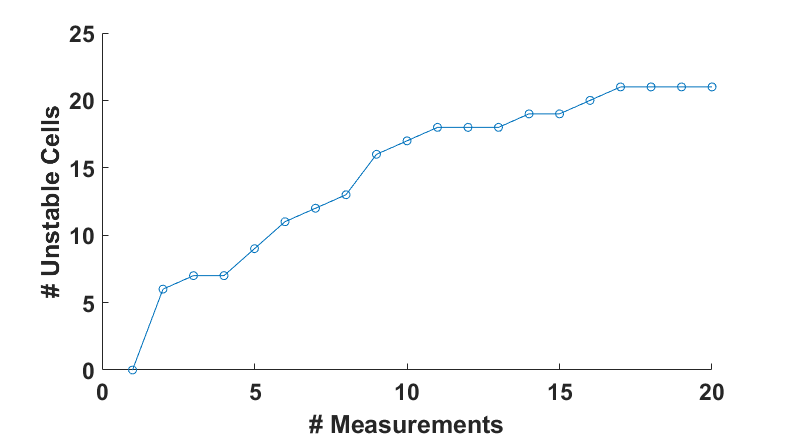
\includegraphics[width=14cm]{images/MEunstable_progression.png}
    \caption{Number of unstable SRAM cells with respect to the number of power-ups.}
    \label{fig:MEunstable_progression}
\end{figure}




\begin{figure}[H]
    \centering
    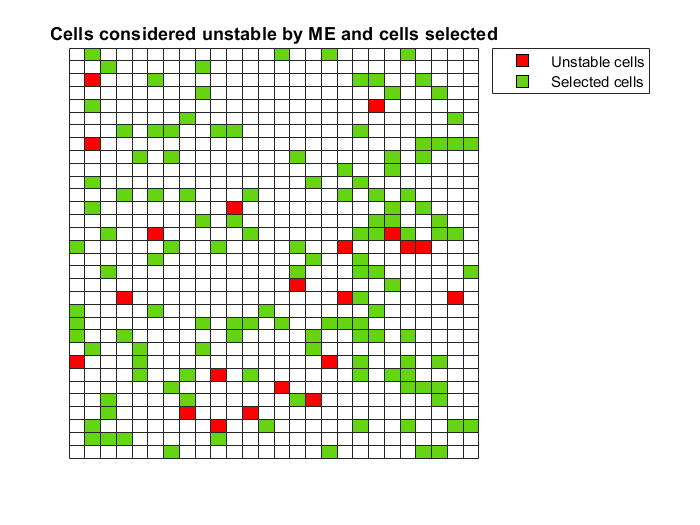
\includegraphics[width=14cm]{images/MEselection.png}
    \caption{Cell-wise representation of the bit selection performed through ME. Cells in red are those considered unstable and cells in green are those selected randomly among the rest.}
    \label{fig:MEselection}
\end{figure}

\subsection{Maximum trip supply voltage selection}

 MTSV selection is explored in detail in section \ref{sec:MTSV}. First, cells that are labelled as unstable due to random behavior during characterization are discarded. These cells are shown in red in fig. \ref{fig:unstable_all}. There are 48 in total, more than double compared to ME. Of the 21 cells labelled as unstable by ME, 17 are also labelled as unstable by MTSV (shown in black), i.e. 80\%. The 4 cells labelled as unstable by ME but not by MTSV (shown in blue) are assigned a low DRV value compared to the rest, so they will be considered weak cells and not form part of any reasonably sized selection. In this way, MTSV discards the cells that ME considers unstable and expands on that considerably.  
 
 \begin{figure}[H]
    \centering
    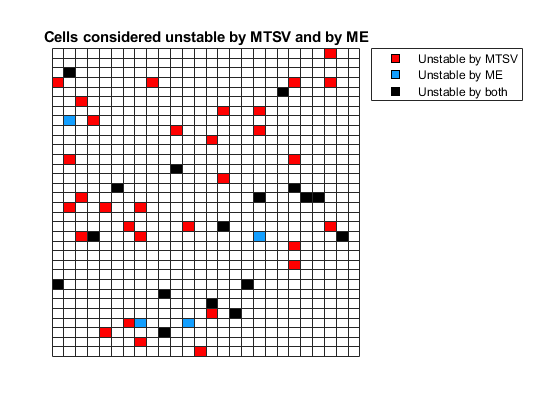
\includegraphics[width=14cm]{images/unstable_all.png}
    \caption{Cell-wise representation of the cells classified as unstable by ME or MTSV.}
    \label{fig:unstable_all}
\end{figure}
    


Then, cells are classified according to their DRV value. The 128 cells with the highest value are selected, which results in the selection \textit{MTSV Strongest}. Another possible scheme to have perfect uniformity is to select the 64 strongest cells biased to ``1'' and the 64 strongest cells biased to ``0'' since the preferred value of each cell is evaluated at enrollment. This selection is called \textit{MTSV Balanced}. The bits selected by either one are shown in fig \ref{fig:MTSVselection}. Cells in red are those considered unstable, cells in blue correspond to \textit{MTSV Strongest}, cells in purple to \textit{MTSV Balanced} and cells in green to both selection. The selections are very similar, differing only in about 10\% of cells. 

\begin{figure}[H]
    \centering
    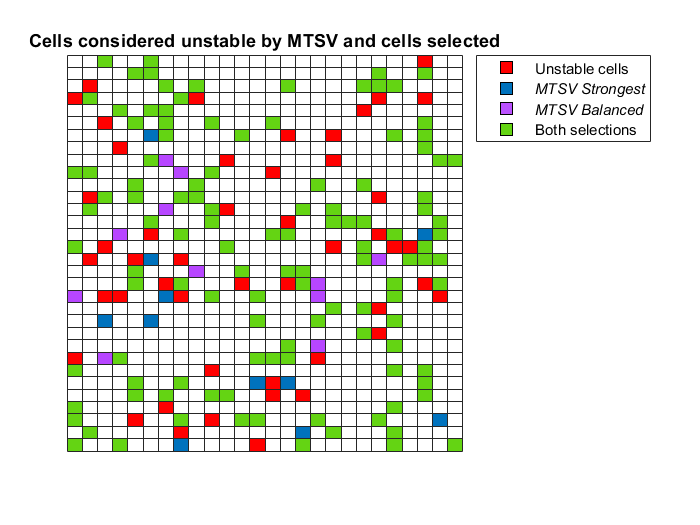
\includegraphics[width=14cm]{images/MTSVselection.png}
    \caption{Cell-wise representation of the bit selection performed through MTSV.}
    \label{fig:MTSVselection}
\end{figure}







\section{Nominal conditions}

Nominal conditions mean room temperature around $\SI{25}{\degree C}$ and a supply voltage of $\SI{1.2}{V}$. Multiple tests with a varying number of power ups for all cells were performed. The results can be found in Table \ref{tab:Nom}. BER and MAXintraHD are calculated intrinsically, i.e. using each dataset as its own reference. 

% in the range of $\SI{22}{\degree C}$ to $\SI{27}{\degree C}$

\begin{table}[H]
  \centering
  \caption{Performance of all cells under nominal conditions.}
    \begin{tabular}{|c|c|c|c|}
    \hline
    Measurements & BER(\%)   & MAXintraHD(\%) & Hamming Weight(\%) \bigstrut\\
    \hline
    200   & 0.4140 & 1.0830 & 50.83 \bigstrut\\
    \hline
    200   & 0.5102 & 1.0830 & 50.94 \bigstrut\\
    \hline
    200   & 0.4693 & 1.2034 & 50.84 \bigstrut\\
    \hline
    1000  & 0.4716 & 1.0830 & 50.94 \bigstrut\\
    \hline
    2000  & 0.5221 & 1.4440 & 51.03 \bigstrut\\
    \hline
    \end{tabular}%
  \label{tab:Nom}%
\end{table}%

BER varies between a value of 0.4140\% and 0.5221\%. This is for multiple tests and stays in a reduced bracket of values for a statistical metric. These values for nominal conditions are considerably low compared to other SRAM PUFs. In \cite{Schrijen2012}, seven different commercial and research SRAM designs are tested under nominal conditions as well as temperature and supply voltage variations.  BER values go between 2.8\% and 4.8\% for nominal conditions in these tests. However, our results are still far away from the desired reliability.

Maximum intra hamming distance is low, with the highest value obtained for the 2000 measurements of 1.444 \%. Hamming weight indicates a very slight bias towards one (Values between 50.83 \% and 51.03 \%), which is an acceptable range. Since the 2000 measurements are the most complete set they will be the ones used from this point onwards as measurements under nominal conditions and to obtain the chip's golden response. One interesting representation is the distribution of BER across the array to see if it follows any spatial pattern. This is shown in fig. \ref{fig:BER_2000_Nom}, and there is no noticeable pattern. It seems clear that most of the errors come from a few cells. Another useful cell-wise representation shown in fig. \ref{fig:p_2000_Nom} is the probability of each cell to power-up as either ``1'' or ``0'', obtained from the approximation of eq. \ref{eq:prob}.


 \begin{figure}[H]
    \centering
    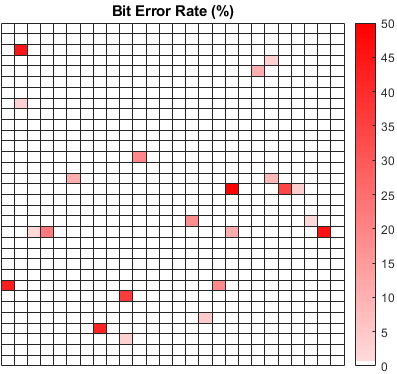
\includegraphics[width=7cm]{images/BER_2000_Nom.png}
    \caption{Cell-wise  representation of BER for the 2000 measurements under nominal conditions. }
    \label{fig:BER_2000_Nom}
 \end{figure}

% Most of the cells with a noticeable BER in fig. \ref{fig:BER_2000_Nom} are labelled as unstable. Cells with a BER of 0 \% under nominal condition are too. This may seem contradictory, but it is important to consider that cells that may appear stable under nominal conditions can be unstable under worse conditions. 



\begin{figure}[H]
    \centering
    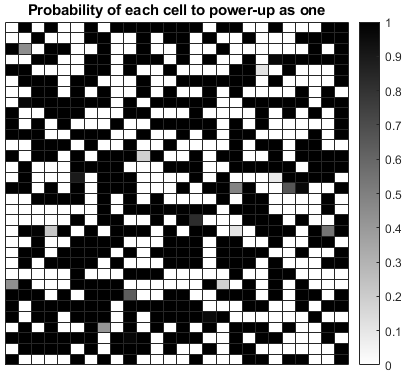
\includegraphics[width=7cm]{images/p_2000_Nom.png}
    \caption{Probability of each cell to power up as ``1'' based on 2000 measurements under nominal conditions. }
    \label{fig:p_2000_Nom}
\end{figure}

Again, no spatial pattern is observed and the distribution of values appears random.  

The performance of the selections presented before under nominal conditions is now examined. BER, maximum intra hamming distance and hamming weight are considered in Table \ref{tab:nom_selections}.

\begin{table}[H]
  \centering
  \caption{Performance of different selections of 128 bits when performing 2000 power-ups under nominal conditions.}
    \begin{tabular}{|c|c|c|c|}
    \hline
    Selection& BER(\%)   & MAXintraHD(\%) & Hamming Weight(\%) \bigstrut\\
    \hline
   \textit{First}& 0.4625 & 2.3438 & 48.07 \bigstrut\\
    \hline
    \textit{Random} & 0.6398 & 3.1250 & 45.11 \bigstrut\\
    \hline
    \textit{ME Stable} & 0.0227 & 0.7813 & 52.32 \bigstrut\\
    \hline
    \textit{MTSV Strongest} & 0.0012 & 0.7813 & 41.41 \bigstrut\\
    \hline
    \textit{MTSV Balanced} & 0.0012 & 0.7813 & 50 \bigstrut\\
    \hline
    \end{tabular}%
  \label{tab:nom_selections}%
\end{table}%

As expected \textit{First} and \textit{Random} have BER values similar to the ones shown in Table \ref{tab:Nom}. Their maximum intra hamming distance is higher due to taking a smaller sample size. \textit{ME Stable} shows a substantial improvement over the values shown in Table \ref{tab:Nom}. BER has reduced from around 0.4-0.6 \% to 0.0227 \%. Hamming weight indicates a result close to uniform, with 52.32 \%. For \textit{MTSV Strongest} and \textit{MTSV Balanced}, BER is reduced even more, going as low as 0.0012 \%. This is one order of magnitude better than \textit{ME Stable}, proving the advantages of the proposed method. 

It is important to keep this very small value for BER in perspective. 2000 power-ups per cell amount to $\SI{2.56}{\cdot 10^5}$ total power-ups for 128 cells. According to eq. \ref{eq:BER}, there were 3 total erroneous power-ups out of  $\SI{2.56}{\cdot 10^5}$. However, these BER values are still not good enough to meet the target of $\SI{7.8}{\cdot 10^{-7}\ \%}$.

Regarding uniformity, there is a significant bias in favor of cells that have ``0'' as a preferred value for \textit{MTSV Strongest}. A hamming weight of around 41 \% is 10\% lower than the hamming weight for all cells. This could be due to the cells' layout, although it is fully symmetric. At this moment, this is an open topic that needs investigation. Further experiments and research are being performed to explain this difference. 

\textit{MTSV Balanced} solves this issue, which is important to avoid leakage of information by the helper data. Hamming weight naturally indicates perfect uniformity at 50 \%. BER is the same as with \textit{MTSV Strongest}, so taking this selection would not come at a significant cost in reliability, at least under nominal conditions. 


\section{Environmental variations}

For measurements under environmental variations, only BER is considered since it is the most relevant metric for reliability.  200 power-ups were performed for each cell at each environmental condition. This is significantly lower than the 2,500 performed in the last chapter due to the fact that 832 cells are evaluated in each case, not just 100. 

\subsection{Resilience to supply voltage variations}

In this set of measurements, cells were powered up 200 times at room temperature and different supply voltages, i.e., raising their supply voltage from ground (\SI{0}{V}) to \SI{1.08}{V}, \SI{1.14}{V}, \SI{1.26}{V} and \SI{1.32}{V}. This corresponds to a range of the nominal voltage $1.2 \ \mathrm{V} \pm 10\%$. 

\begin{table}[H]
  \centering
  \caption{Mean BER value for the different selections when performing 200 power-ups under supply voltage variations}
    \resizebox{\linewidth}{!}{%
    \begin{tabular}{|c|c|c|c|c|c|c|}
    \hline
    $V_{DD}$ (V)   & All  & \textit{First} & \textit{Random} & \textit{ME stable} & \textit{MTSV Strongest} & \textit{MTSV Balanced} \bigstrut\\
\hline
1.08   & 0.5355 & 0.3164 & 0.9492 & 0.1172 & 0.0078 & 0.0078 \bigstrut\\
\hline
1.14   & 0.5788 & 0.4023 & 1.0469 & 0.1406 & 0     & 0 \bigstrut\\
\hline
1.26   & 0.6444 & 0.3555 & 1.0117 & 0.043 & 0     & 0 \bigstrut\\
\hline
1.32   & 0.7148 & 0.375 & 1.0508 & 0.0391 & 0.0039 & 0.0039 \bigstrut\\
\hline
\end{tabular}%
}
  \label{tab:vdd_sel}%
\end{table}%

BER increases slightly as $V_{DD}$ increases according to this data. The change in reliability is not very significant, as expected. The worst BER is obtained for a supply voltage of \SI{1.32}{V}. Bit selection techniques show a similar improvement to the one done under nominal conditions. \textit{MTSV Strongest} and \textit{MTSV Balanced} show low errors so these selections are robust under supply voltage variations. 



\subsection{Resilience to temperature variations}

% Table generated by Excel2LaTeX from sheet 'General analysis'
\begin{table}[b]
\small
  \centering
  \caption{Mean BER value for the different selections when performing 200 power-ups under temperature variations}
  \resizebox{\linewidth}{!}{%
    \begin{tabular}{|c|c|c|c|c|c|c|}
    \hline
    T (°C) & All & \textit{First} & \textit{Random} & \textit{ME stable} & \textit{MTSV Strongest} & \textit{MTSV Balanced} \bigstrut\\
    % Table generated by Excel2LaTeX from sheet 'General analysis'
\hline
-20  & 2.4272 & 2.2578 & 1.6641 & 0.0117 & 0.039 & 0.0039 \bigstrut\\
\hline
0    & 1.3267 & 0.8125 & 0.9844 & 0     & 0     & 0 \bigstrut\\
\hline
10   & 0.9344 & 0.5234 & 0.9844 & 0.0078 & 0     & 0 \bigstrut\\
\hline
20   & 0.8057 & 0.3789 & 0.9766 & 0.0195 & 0     & 0 \bigstrut\\
\hline
40   & 0.9615 & 0.7656 & 1.2734 & 0.3711 & 0     & 0 \bigstrut\\
\hline
\end{tabular}%
}
  \label{tab:temp_sel}%
\end{table}%

In these tests, instead of using the ACS climatic chamber employed in the previous chapter, a Thermonics T-2650BV is used. It allows for a larger range of temperatures by setting a determined temperature for the IC chip without affecting the whole PCB. 200 power-ups were performed for each cell, at $\SI{-20}{\degree C}$, $\SI{0}{\degree C}$, $\SI{10}{\degree C}$, $\SI{20}{\degree C}$ and $\SI{40}{\degree C}$. The resulting BER is shown in Table \ref{tab:temp_sel}. Measurements at higher temperature were attempted, but the results did not agree with the expected value found in literature and simulations. More experiments were planned, but the Thermonic T-2650BV broke down, and they could not be performed.





The changes in BER due to temperature variations are more noticeable. As temperature deviates from $\SI{20}{\degree C}$ upwards or downwards, BER increases. From $\SI{-20}{\degree C}$ to $\SI{40}{\degree C}$,  \textit{MTSV Strongest} and \textit{MTSV Balanced} selections are able to provide  practically error free results. 

% However, for $\SI{60}{\degree C}$ and specially $\SI{80}{\degree C}$ BER becomes too high and ME or MTSV bit selection does not seem to improve reliability significantly. This is because at these temperatures all cells biased to ``0'' present at least one bitflip, i.e. they are biased to be more unstable, while cells biased to ``1'' remain mostly stable. This is clearly shown in figure \ref{fig:p_200_80C}, where there are no cells in white. 

% \begin{figure}[H]
%     \centering
%     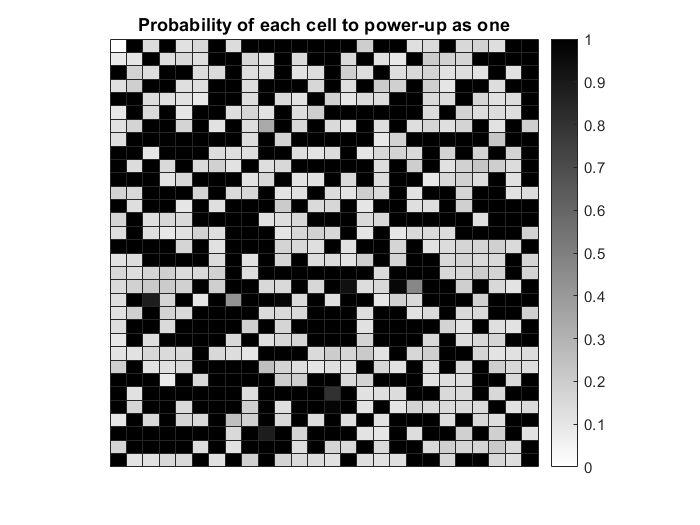
\includegraphics[width=13cm]{images/p_200_80C.png}
%     \caption{Probability of each cell to power-up as ``1'' based on 200 measurements at $\SI{80}{\degree C}$.}
%     \label{fig:p_200_80C}
% \end{figure}

% The cell-wise BER for the 200 measurements at $\SI{80}{\degree C}$ is represented in fig. \ref{fig:BER_80C}. A general increase of the BER value in the array is observed, although some cells considered unstable at room temperature are now more stable. Actually, both behaviours (increase and decrease of stability with temperature) have been confirmed through simulation and depend on the mismatch of the PMOS and NMOS transistors of the cell. In the literature there are reported studies that confirm a similar degradation of the BER values with temperature \cite{Schrijen2012}, with average BERs for different devices going from 6.6\% to 10.5\% for $\SI{80}{\degree C}$, although proportionally the increase is much smaller.

% \begin{figure}[H]
%     \centering
%     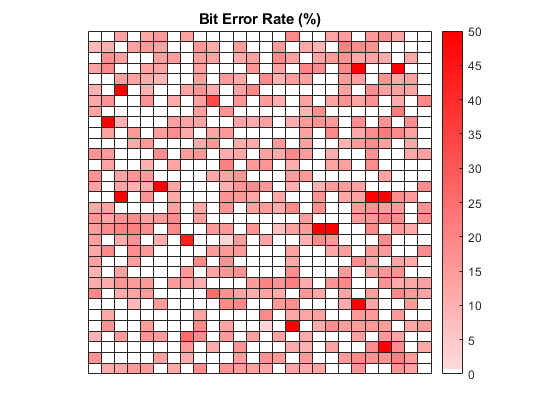
\includegraphics[width=12cm]{images/BER_80_C.png}
%     \caption{Cell-wise representation of BER for 200 measurements at $\SI{80}{\degree C}$. }
%     \label{fig:BER_80C}
% \end{figure}


% Evaluating the hamming weight of all cells at different temperatures the decrease in reliability of cells biased to ``0'' can be quantified. At $\SI{40}{\degree C}$, hamming weight is 50.51 \%, close to uniform. However, at  $\SI{60}{\degree C}$ it increases to 51.56 \% and at  $\SI{80}{\degree C}$ it goes up to 57.58 \%. In \cite{Schrijen2012}, changes in hamming weight with temperature are in the order of 1\%, not 7\%. The reason for such a heavy reduction in reliability only for cells biased to ``0'' is unclear, and is presently under study. In principle, the design of SRAM cells is symmetrical so there should not be such a considerable difference between the behaviour of cells biased to ``1'' or ``0''. Measurements performed after this test under nominal conditions show no increase in BER, so there was no permanent damage caused by the high temperature.  
% If this increase was normal, no selection should be able to significantly reduce the BER, which is incoherent with works such as \cite{Liu2017} where the BER is reduced down to 0 \% through a data remanence bit selection technique even for measurements at $80 \degree$C. 

% Observing these results, an attempt to repeat the same experiments on more samples was performed, so that this behaviour could be confirmed. Unfortunately, the thermal equipment used for them (Thermonics T-2650BV) was experiencing working problems during the last months, and definitely broke down just after measurements on chip \#6 were done. Further studies will be performed in the next months when new equipment will be available.  



\subsection{Resilience to circuit aging}

In this section, the procedure described in section \ref{ss:aging} is employed to evaluate the adequacy of the selections for cells under accelerated aging. In this case, all the cells were stressed. The measures performed are right after stress ended, 8 days later and 21 days later. It is important to point out that measurements right after stress are not instantaneous, it takes about 100 seconds to perform the 200 power-ups. The BER for each selection and point in time $t$ are shown in Table \ref{tab:aging_sel}.

\begin{table}[H]
\resizebox{\linewidth}{!}{%
\begin{tabular}{|c|c|c|c|c|c|c|}
\hline
    $t$ & All & \textit{First} & \textit{Random} & \textit{ME stable} & \textit{MTSV Strongest} & \textit{MTSV Balanced} \bigstrut\\
\hline
Before & 0.7858 & 0.6836 & 1.4453 & 0.043 & 0     & 0 \bigstrut\\
\hline
Right after stress & 7.4049 & 6.9492 & 6.4297 & 4.6523 & 1.0586 & 0.8477 \bigstrut\\
\hline
8 Days & 4.7918 & 5.8438 & 4.6914 & 1.9297 & 0.0039 & 0.0039 \bigstrut\\
\hline
21 Days & 4.7136 & 5.1406 & 4.6719 & 1.2227 & 0 & 0 \bigstrut\\
\hline
\end{tabular}%
}
  \caption{Mean BER value for the different selections when performing 200 power-ups at different points in time after accelerated aging.}
  \label{tab:aging_sel}%
\end{table}%

 \vspace*{-\baselineskip}


\begin{figure}[b!]
    \centering
    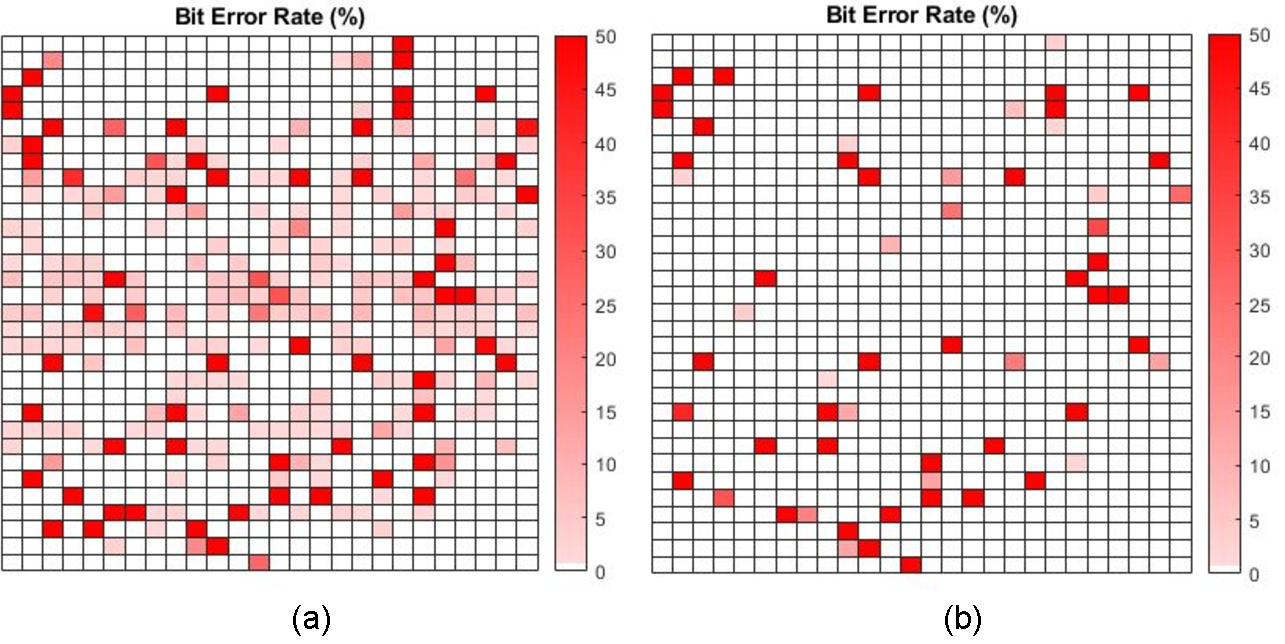
\includegraphics[width=14cm]{images/BER aging comparison.pdf}
    \caption{Cell-wise representation of BER for 200 measurements right after stress (a) and 8 days later (b). }
    \label{fig:BER_aging_comparison}
\end{figure}

The degradation of the cells is quite clear, with BER being around 10 times larger before and after stress for all cells (from 0.7858 \% to 7.4049 \%). \textit{First} and \textit{Random} have values close to \textit{All cells}, as expected. The temporal component of BTI is demonstrated by the decrease of about 3 \% in BER for all cells after 8 days. A measurement 21 days later shows some recovery, but it is considerably smaller. The recovery can be observed graphically by comparing the cell-wise BER right after stress, as shown in fig. \ref{fig:BER_aging_comparison} (a) and 8 days later, as shown in fig. \ref{fig:BER_aging_comparison} (b).  

\textit{ME stable} is capable of reducing the BER by about 3\%, but these values are still high. The results for either MTSV selection are outstanding. Right after stress BER is reduced to 1.0586 \% for \textit{MTSV Strongest} and to 0.8477 \% \textit{MTSV Balanced}. After 8 days it goes down to 0.0039 \% for both of them, and after 21 the selected cells achieve 0\% BER, the value obtained before stress. It clearly shows how MTSV is able to select those cells resilient to aging while the ME technique cannot. 





\section{Complete cryptographic solution}

Once the PUF response has been fully characterized, a complete HDA scheme can be implemented with these measurements. The fuzzy commitment construction explained in section \ref{sec:HDAs} will be employed, where a secret key is obfuscated through the PUF response. To measure the validity of this construction, each time the key is recovered successfully, it will be counted as a success. The Acceptance Rate (AR) will be the number of successful recoveries. In this way, it can range from zero, for no successful recoveries, to the number of attempts, where the key is successfully recovered each time. 

As discussed in chapter \ref{ss:ecc}, there are plenty of choices available as an ECC. Considering the low BER for both MTSV selections, a repetition code seems like the best choice. This code is the simplest to implement, essential for resource-constrained devices, has good error correction capabilities and will not require many bits since BER is already significantly reduced by the selection. To generate a 128-bit key, only two repetition codes use less than 832 bits: $R[3,1,3]$, which uses 384 bits and $R[5,1,5]$, which uses 640. Naturally, new selections are required for these sizes, performed by following the same criteria explained earlier. As MTSV classifies cells according to their strength, a larger selection will have higher BER.   

First, the HDA will be implemented with the power-ups performed under nominal conditions for the different selections. Then, it should be tested in a bad corner for reliability. The measurement right after accelerated aging is not considered, as applying such a high stress for an extended period of time is not realistic in actual implementations. A better approach is to use the measurements at low temperature, $-20 \degree$C, as well as those taken 8 days after accelerated aging, as they have a considerable increase in BER and can be trusted to represent a realistic degradation of reliability. 

Afterwards, one interesting test is to try and recover the key with a response from another chip. There should be an AR of zero, as each PUF is unique. Finally, the theoretical requirements of the repetition code for each scenario based on the BER measurements are examined. 



\subsection{Key generation under nominal conditions}

First, the 2000 power-ups performed under nominal conditions are used to test this construction. The helper data corresponding to each selection and repetition code is generated once (Enrollment) and each one of the 2000 power-ups are employed as individual attempts to recover the key (Reconstruction). The helper data generated during enrollment will be the one used in the other tests.

Results regarding AR are shown in Table \ref{tab:AR_nominal}, where $n$ refers to the parameter of the repetition code. The AR is high for all selections, but it is expected as the number of measurements is low for a BER of around 0.5 \%. In any case, for $R[3,1,3]$, \textit{First} shows one error and \textit{Random} seven. These errors no longer occur if the repetition code is expanded to $R[5,1,5]$, showing how a code with more redundancy has higher error correcting capabilities.   
% To illustrate this procedure with real data, the variables used during the enrollment phase and one reconstruction are shown for the \textit{First} selection and $R[3,1,3]$.

% During enrollment, the PUF response used to obfuscate the data is generated:

% \longstring{1,0,1,0,0,1,0,1,1,1,1,1,1,1,0,1,1,0,0,1,0,0,0,1,1,0,0,1,0,0,0,1,1,0,0,1,0,1,1,0,1,0,0,1,0,0,0,1,1,1,1,1,0,0,1,1,0,0,1,0,0,1,0,0,1,0,0,1,0,0,0,0,0,0,1,0,1,0,0,1,1,0,0,1,1,0,1,1,1,0,1,0,1,0,0,1,0,1,1,1,1,1,1,1,1,0,0,0,0,1,1,0,1,0,0,1,0,0,0,0,1,1,0,0,1,0,0,0,1,0,1,1,1,0,1,1,0,0,0,1,0,0,1,1,1,1,1,1,0,1,0,0,0,0,1,0,0,1,1,0,1,0,1,0,0,1,0,1,0,0,1,0,1,0,0,0,0,1,0,1,0,0,1,1,1,1,1,1,1,0,1,0,1,1,1,1,1,0,0,1,1,1,1,1,0,1,1,1,0,0,1,1,1,0,0,0,1,1,0,0,0,1,0,0,0,0,1,0,1,0,1,0,1,1,0,1,0,1,0,0,0,1,0,0,1,1,1,1,1,0,1,0,1,0,0,0,0,0,1,1,1,1,0,0,1,1,1,0,0,1,0,0,1,0,1,0,1,1,0,0,0,0,1,0,1,0,0,1,1,1,0,1,0,0,1,0,0,1,0,0,0,0,1,0,1,1,0,1,1,0,0,1,0,1,1,0,1,0,1,1,1,0,1,0,0,1,0,1,1,0,0,1,0,1,1,1,1,0,1,0,0,0,1,1,1,1,0,0,0,1,1,1,0,0,1,1,1,1,1,0,1,1,1,0,1,0,0,0,0,0,1,1,1,0,0,0,0,1,0,1,0,0,0,0
% }

\begin{table}[H]
\resizebox{\linewidth}{!}{%
\begin{tabular}{|c|c|c|c|c|c|c|c|c|c|c|}
\hline
 & \multicolumn{2}{c|}{\textit{First}} & \multicolumn{2}{c|}{\textit{Random}} & \multicolumn{2}{c|}{\textit{ME stable}} & \multicolumn{2}{c|}{\textit{MTSV Strongest}} & \multicolumn{2}{c|}{\textit{MTSV Balanced}} \bigstrut\\
\hline
$n$     & 3 & 5 & 3 & 5 & 3 & 5 &  \ \ \ \  3  \ \ \ \  & 5 &  \ \ \ \  3  \ \ \ \ & 5 \bigstrut\\
\hline

Required bits     & 384 & 640 & 384 & 640 & 384 & 640 &  384 & 640 &  384 & 640 \bigstrut\\
\hline
BER (\%)  & 0.2622 & 0.5447 & 0.6023 & 0.4178 & 0.0164 & 0.0133 & 0.0007 & 0.0016 & 0.0007 & 0.0016 \bigstrut\\
\hline
AR    & 1999 & 2000 & 1993 & 2000 & 2000 & 2000 & 2000 & 2000 & 2000 & 2000 \bigstrut\\
\hline
\end{tabular}%
}
  \caption{BER and AR value for the different selections when performing 2000 power-ups under nominal conditions using two different repetition codes.}
  \label{tab:AR_nominal}%
\end{table}%

\subsection{Key generation at low temperature}

 For $\SI{-20}{\degree C}$ less power-ups were performed, 200, so the AR will go up to that value. Results are shown in Table \ref{tab:AR_-20C}. There are more erroneous responses this time, specially considering how the number of power-ups is 10 times lower. It is clear how the decrease in reliability, i.e. the increase in BER, translates into a decrease in AR, and why considering only measurements under nominal conditions is not enough. Only \textit{MTSV Balanced} is able to recover the key 200 times for $R[3,1,3]$. There is one specific power-up with a larger number of bit-flips, due to the statistic nature of this process. This power-up is enough to cause one error in most selections. Even after applying a $R[5,1,5]$ only the selections based on MTSV are able to recover the key, showing once again its advantages versus multiple evaluation. 


\begin{table}[H]
\resizebox{\linewidth}{!}{%
\begin{tabular}{|c|c|c|c|c|c|c|c|c|c|c|}
\hline
 & \multicolumn{2}{c|}{\textit{First}} & \multicolumn{2}{c|}{\textit{Random}} & \multicolumn{2}{c|}{\textit{ME stable}} & \multicolumn{2}{c|}{\textit{MTSV Strongest}} & \multicolumn{2}{c|}{\textit{MTSV Balanced}} \bigstrut\\
\hline
$n$     & 3     & 5     & 3     & 5     & 3     & 5     & \ \ \ \  3  \ \ \ \  & 5 &  \ \ \ \  3  \ \ \ \     & 5 \bigstrut\\
\hline
Required bits     & 384 & 640 & 384 & 640 & 384 & 640 &  384 & 640 &  384 & 640 \bigstrut\\
\hline
BER (\%)   & 1.5299 & 2.1696 & 3.4792 & 2.1273 & 0.7643 & 1.4500  & 0.0143 & 0.2203 & 0.0938 & 0.2453 \bigstrut\\
\hline
AR    & 198  & 199  & 60  & 199  & 199  & 199 & 199  & 200  & 200  & 200 \bigstrut\\
\hline
\end{tabular}%
}
  \caption{BER and AR value for the different selections when performing 200 power-ups at $\SI{-20}{\degree C}$ using two different repetition codes.}
  \label{tab:AR_-20C}%
\end{table}%

\subsection{Key generation after accelerated aging}

As in the previous test, 200 power-ups are employed. The AR obtained for each selection and repetition code is shown in Table \ref{tab:AR_aging}. In this case, except for \textit{First} and \textit{Random} for a repetition code $R[3,1,3]$, the key is recovered successfully each time. This may seem counter-intuitive considering how AR was lower in the previous test while BER is higher in this one. However, it is explained by considering that the way BER is distributed matters greatly for key generation. In the previous test, there was one power-up that showed more bit-flips. Out of 200 power-ups, it does not have a large impact in the average BER, but it does translate in one failure to recover the key. 

\begin{table}[H]
\resizebox{\linewidth}{!}{%
\begin{tabular}{|c|c|c|c|c|c|c|c|c|c|c|}
\hline
 & \multicolumn{2}{c|}{\textit{First}} & \multicolumn{2}{c|}{\textit{Random}} & \multicolumn{2}{c|}{\textit{ME stable}} & \multicolumn{2}{c|}{\textit{MTSV Strongest}} & \multicolumn{2}{c|}{\textit{MTSV Balanced}} \bigstrut\\
\hline
$n$  & 3     & 5     & 3     & 5     & 3     & 5     & 3     & 5     & 3     & 5 \bigstrut\\
\hline
Required bits     & 384 & 640 & 384 & 640 & 384 & 640 &  384 & 640 &  384 & 640 \bigstrut\\
\hline
BER (\%)   & 4.4766 & 4.5484 & 5.4375 & 4.7492 & 2.8672 & 3.7188 & 0.0482 & 1.0211 & 0.0482 & 0.9695 \bigstrut\\
\hline
AR    & 186   & 200     & 139   & 200     & 200     & 200     & 200     & 200     & 200     & 200 \bigstrut\\
\hline
\end{tabular}%
}
  \caption{BER and AR value for the different selections when performing 200 power-ups 8 days after accelerated aging using two different repetition codes.}
  \label{tab:AR_aging}%
\end{table}%

\subsection{Key generation using other chips}

In this test, an attempt to recover the key with a different chip is performed. To do this, the helper data generated under nominal conditions for this chip is used in combination with the 200 power-ups measured for each of the five chips employed in the previous chapter, resulting in 1000 power-ups to work with. For any selection or repetition code, the AR obtained is 0, showing that a chip cannot be used to recover the key obfuscated by another chip. This verifies the uniqueness of the PUF, although on a small scale since only 6 chips are used in total.


\subsection{Repetition code requirements for low KER}

So far, different repetition codes have been tested with real measurements. However, the target for KER was set at $10^{-4}$ \%. It is important to remember that this means around one error per million attempts. In our measurements, the largest number of power-ups performed was 2000 under nominal conditions, and to verify that the KER target is met with statistical significance power-ups in the order of a million would be required at a bad corner of reliability, which is not feasible. 
Instead, the error reduction capabilities of the repetition code can be estimated using the binomial distribution (equation \ref{eq:binomialpmf}).  Since more than half of the bits need to fail, the probability of failure after the repetition code will be the cumulative probability $P\left(x\geq \frac{n+1}{2}\right)$ for $p=\mathrm{BER}$ and $R[n,1,n]$. This probability can be calculated through MATLAB, and the lowest $n$ that meets the requirements is chosen. To differentiate the two stages, $\mathrm{BER}_0$ is the BER before applying an ECC and $\mathrm{BER}_F$ the BER after ECC. As a reminder, the target $\mathrm{BER}_F$ is $\SI{7.8}{\cdot 10^{-7}\ \%}$ for a KER of $10^{-4} \%$. 

Leaving out the measurements performed right after applying stress and taking the values for 128-bit selections, the worst case for each selection is a BER of 5.8438 \% for \textit{First}, 4.6914 \% for \textit{Random} and 1.9297 \% for \textit{ME Stable}, where these three values were obtained in the aging test 8 days after accelerated aging and 0.0078 \% for both \textit{MTSV Strongest} and \textit{MTSV Balanced}, obtained in the supply voltage test for 1.08 V. Since both \textit{MTSV Strongest} and \textit{MTSV Balanced} have the same $\mathrm{BER}_0$, they will be simply referred as \textit{MTSV} from now on. The results of this procedure are shown in Table \ref{tab:rep}.

 
 
 
 \begin{table}[H]
\resizebox{\linewidth}{!}{%
\begin{tabular}{|c|c|c|c|c|c|}
\hline
    Selection & $\mathrm{BER}_0$ (\%) & $C$ & $\mathrm{BER}_F$ (\%)& KER (\%)& PUF bits \bigstrut\\
\hline
\textit{First} & 5.8438 & $R[21,1,21]$ & 5.53 E-7 & 7.07 E-5 & 2688      \bigstrut\\
\hline
\textit{Random} & 4.6914 & $R[19,1,19]$  & 3.22 E-7 & 4.13 E-5 & 2432  \bigstrut\\
\hline
\textit{ME Stable} & 1.9297 & $R[13,1,13]$ & 1.54 E-7 & 1.93 E-5 & 1644  \bigstrut\\
\hline
\textit{MTSV} & 0.0078 & $R[5,1,5]$  & 4.75 E-10 & 6.07 E-8 & 640  \bigstrut\\
\hline
\end{tabular}%
}
  \caption{Required repetition code to meet the KER target for each selection.}
  \label{tab:rep}%
\end{table}%

The predicted reduction in required redundant bits is made apparent with these results. \textit{First} and \textit{Random} require a large amount of redundant bits, 2688 and 2432 bits respectively. While for \textit{ME Stable} the required bits are reduced significantly, down to 1644, it is still a large number. The repetition code is perhaps not ideal for these selections, but as seen in Table \ref{tab:ECCs} there is a limit on how efficient the code may be with higher complexity. For \textit{MTSV}, a $R[5,1,5]$ code will achieve a KER of $\SI{6.07}{\cdot 10^{-8}\ \%}$, considerably lower than the rest. The required bits are significantly reduced. These results are consistent with the measurements at low temperature, where only a MTSV based selection with $R[5,1,5]$ is able to recover the key successfully each time. 
 
 
%  Based on the results, two scenarios are going to be considered: \textit{Optimistic} and \textit{Pessimistic}. According to \textit{Pessimistic}, the worst corner measured is the one used as reference for the KER, as the PUF is expected to have a good response under the complete range of possible environmental conditions. This would clearly be the measurement taken for $80 \degree C$, where BER goes from around $7\%$ to $10\%$. However, as explained before, this BER is very high due to the fact that every cell biased to zero becomes unstable, which is unexpected in SRAM PUF cells. If this is the case, no selection should be able to significantly reduce the BER, which is incoherent with works such as \cite{Liu2017} where the BER is reduced down to 0 \% through a data remanence bit selection technique even for measurements at $80 \degree$C. 

% The other possible scenario is \textit{Optimistic}. The results for $60 \degree$C and $80 \degree$C are not considered due to the massive drop in reliability for cells biased to ``0'' uncharacteristic of SRAM PUFs. For the aging test the measurements after 8 days are used as reference, since in real applications the PUF will not be powered on permanently and will have time to recover from BTI degradation. Leaving out these three measurements, the worst case for each selection is a BER of 5.8438 \% for \textit{First}, 4.6914 \% for \textit{Random} and 1.9297 \% for \textit{ME Stable}, where these three values were obtained in the aging test 8 days after accelerated aging and 0.0078 \% for both \textit{MTSV Strongest} and \textit{MTSV Balanced}, both obtained in the supply voltage test for 1.08 V. Since both \textit{MTSV Strongest} and \textit{MTSV Balanced} have the same $\mathrm{BER}_0$, they will be simply referred as \textit{MTSV} from now on.

% Out of these two possible scenarios \textit{Optimistic} is chosen, since it provides a fairer comparison between selections which is the objective of this work. Considering the results obtained here and those present in the bibliography \cite{Liu2017,Schrijen2012}, a MTSV selection is expected to perform in line with the rest of tests for high temperatures in chips with different design. This assertion would need to be verified and is part of possible future work. 














 
 
 
 

% \section{Measurements: results and discussion}
% All of these metrics are tested for a variety of PUF measurements datasets obtained from different KIPT chips \cite{kipt}. They were done to verify the validity of the Maximum Trip Supply Voltage (MTSV) technique \cite{mtsv}, explained in detail in the next subsection. It's goal is to classify cells regarding their stability to improve the PUF's reliability. KIPT is a chip designed in UMC 65-nm CMOS technology for the characterization of aging and RTN effects on IC circuit blocks. Among other elements it has an array of 832 SRAM cells used for PUF-related tests, the one of interest in this case. These measurements include raw power-up data as well as tests where different operating parameters are modified. The validity of the MTSV technique is confirmed first under nominal conditions and specially after temperature and supply voltage variations as well as forced aging.  The metrics are implemented in MATLAB. In eachTableof data $m$ is the number of power-ups per cell performed in each case. 

% \subsection{Nominal characterizations}
% In the first place the nominal characterizations are considered. In these the golden response is obtained intrinsically, since they are the fresh characterizations used later as reference. These can be observed in Table \ref{tab:nom}. Measurements have been performed on two different sets of cells:
% \begin{itemize}
%     \item All the 832 cells in the array (All)
%     \item 50 strongest and 50 weakest cells among those considered stable by Maximum Trip Supply Voltage (SnW)
% \end{itemize}

% MTSV works as follows: Suppose a cell has a certain preferred value. If the cell is storing its non-preferred value and the supply voltage is gradually reduced, there will be a point where the value will flip. Accordingly, the sooner it flips the stronger the bias to the preferred value. This can be used to have a direct measurement on how stable the cell is. Cells that flip more than once during the supply voltage variation are considered unstable and are discarded and the rest are ranked from strongest to weakest according to their MTSV. The traditional method to determine stability was simply multiple evaluation \cite{Baturone2015}, i.e. measuring the PUF multiple times under nominal conditions and keeping the cells that have the same outcome more consistently. 

% Regarding reliability, using MTSV to clasify cells consistently reduces BER and makes the minimum entropy closer to 0 for both strong and weak cells, indicating more stability. Values can be compared in Table \ref{tab:nom}. Maximum intra hamming distance tends to increase, with values being around 1-2 \% for the whole array of cells and 4-8\% for SnW cells. This metric depends on the length of the response and the difference in the probabilistic outliers. Accordingly, it could be that decrease in length has more weight than the reduction of outliers from the preselection, even if the overall BER is improved. However, the fact that many more powerups were performed for SnW (from 2500 to 3700) than for all cells (200 in all chips) is probably the reason for a higher intraHD. Many more pairs of responses are compared for SnW and outliers will be more frequent the higher the samples. Generally the classification between strongest and weakest cells seems to work properly, with BER, MAXintraHD and minimum entropy being lower which indicates more reliability. There is one exception with chip 1, where BER and entropy are slightly higher for the strongest cells. This could be a statistical outlier and be caused by the fact that all cells considered stable have high reliability. It has to be considered that MTSV shines versus Majority Vote when operating conditions change, not so much in nominal conditions. 

% Upon examination of the hamming weight, it is clear that cells biased to 0 tend to be more stable, while those considered weakest tend towards 1 in all chips. Exact values across chips vary in a wide range from 0,32 to 0,44 for the strongest cells and from 0,60 to 0,68. The strongest cells have a hamming weight far from the ideal 0,5, which means that uniformity could be a problem when using MTSV to classify cells. The origin of this correlation between bias to 0 and stability is uncertain. It could be inherent to this metric or caused by the chip's design. This method should be employed in other designs to investigate further. The values for all cells are acceptable, close to 0,5 but with sizeable variation. Some are lower than 0,5 but there seems to be a slight tendency towards cells biased to one. The sample size isn't big enough to affirm it. 



% \subsection{Performance tests}
% In the following tests metrics were determined extrinsically by comparing power-up values of the 50 Strongest and 50 Weakest cells according to MTSV to their corresponding golden responses generated from the nominal characterizations explained before. 
% \subsubsection{Temperature variations}
% The first test was performance under temperature variations for chip 8, in a range from $0\degree$ to $40\degree$. Results are shown in Table \ref{tab:Temp}. Weakest cells perform better under the standard condition of 20$\degree$ and worse for lower and specially higher temperatures, with lower reliability and uniformity. Strongest cells remain stable through the range of temperatures. 
% \subsubsection{\texorpdfstring{$V_{dd}$}{Vdd} variations}
% The second test was to observe the stability of the response to supply voltage variations. The nominal value of the supply voltage is 1,2 V. A generous margin is to estimate possible variations as 10\% of this value, i.e. from 1,08 V to 1,32 V. It would seem like a voltage below the nominal value doesn't have a noticeable effect on reliability as observed in Table \ref{tab:Vdd}. For values above it the weakest cells seem to perform worse while the strongest remain stable once again, validating the MTSV classification. Uniformity isn't affected in either weak or strong cells. 
% \newpage
% \subsubsection{Circuit aging}
% In the third test aging is evaluated. First, the preferred value is written and stored at a high supply voltage (2.5 V) for 10000 s. This reinforces the non-preferred value due to bias temperature instability (BTI) CITE PREVIOUS CHAPTER. This kind of degradation has a permanent and a temporal component. To test it, measurements were performed at different dates.

% Strongest cells are not noticeably affected by this stress  as seen in Table \ref{tab:evolution}. Weakest cells however turn very unstable. Their tendency  is to ``regenerate'' themselves with time due to the temporal component of the degradation wearing off. In terms of uniformity the hamming weight of the weakest cells increases with stress but interestingly enough it increases even more as time goes by. 
% \subsection{Strongest 256 bits implementation}

% In real application scenarios nowadays cryptographic keys usually have 256 bits. An array with many times more cells than KIPT would be employed and the selection of 256 cells would represent a smaller percentage of the total cells. Accordingly, results should be better since there would be a higher number of cells from which to pick the best ones. It is interesting anyways to test how good this array would be when selecting the strongest 256 bits. Complete measurements of MTSV and all chips were performed for four chips, results of applying metrics to those can be found in Table \ref{tab:stable}. BER is still quite low and reliability is satisfactory and comparable to the previous measurement of the strongest 50 cells. Since more cells are selected uniformity improves, with a better hamming weight. It's closer to 0,5 but strong cells are still strongly biased to 0. 
% \subsection{Uniqueness}

% Since uniqueness is measured comparing responses across different chips, inter hamming distance values are separated from the rest and can be found in Table \ref{tab:inter}. The 256 strongest cells selection is used for the comparison because, as explained before, it emulates real application scenarios better. This means that only four chips are used which is a small sample size, so results are not definitive. To illustrate the hamming distance measurement process and since there are few possible pairs, the hamming distance between all pairs is shown. These values can be found in Table \ref{tab:inter}, and are averaged to obtain the inter hamming distance. Results for all cells are good, close to 50\% and with a clear tendency towards values lower than it. In the 256 cells, the result is a perfect 50\% for the mean. Examining each of the pairs, there is a sizeable variability in the HD of each pair going above and below 50\%. Such a good result is probably radom chance and a consequence of the small sample size, but it shows that in any case uniqueness should be within acceptable margins.  
% \newpage
% \subsection{True Random Number Generator}
% Lastly, the capability of the PUF to generate random numbers through the MTSV method is evaluated. In this case, the metric of most interest is entropy, the higher it is the better the result. It doesn't make sense to compare the metrics of a TRNG to an ideal string since the objective isn't to generate an unique identifier, so they are measured intrinsically. MTSV can be employed to create the TRNG as well. Suppose a cell is written with its non preferred value. Then, the voltage is decreased to the trip voltage of the cell, i.e., the voltage at which it flipped from its non-preferred to its preferred value at the MTSV procedure. Further measurements done at the trip voltage by this 
% method will be unpredictable since they are around the frontier between two outputs and a small variation can cause it to go one way or the other. The smaller the step is when determining this voltage the closer it will be to the actual frontier. Accordingly, the entropy and thus randomness will be higher which can be observed in Table \ref{tab:MTSV}. Reducing the step voltage would come at a cost in computation and hardware specifications. The results using all cells for this chip are included again in the last row for comparison. 

% Another method to have a TRNG using the MTSV would be to employ those cells that were discarded due to being unstable. This is similar to the method applied in \cite{Baturone2015}, where cells considered unstable through majority vote are used to generate random numbers. The result of employing cells considered unstable by MTSV is shown in Table \ref{tab:usntable}. The number of unstable cells $n$ is different in each case. The minimum entropy measured using those is considerable, ranging from 11\% to 22\% (High variability). This is comparable to using a step size of 2 mV in the previous case. The drawback is that the number of cells employed is much lower, whereas with the prior method all cells in the array are used. However, if a large number of cells are available in a bigger array, this method comes at no cost in computation or hardware specifications. Uniformity is important as well for a TRNG and the proposed MTSV method has better values, with a HW reasonably close to 0,5\% while using unstable cells leads to choosing cells biased strongly towards either 0 or 1.
% \newpage
% \subsection{Bias from MTSV and state-wise performance}

% The uniformity of the response can be checked with the hamming weight. In Table \ref{tab:256Strongest} bit error rate and hamming weight from 200 evaluations of the best 256 cells according to MTSV under nominal conditions are shown. The hamming weight has a clear tendency towards ``0'' in all chips. If MTSV works properly, this would indicate that cells biased to ``0'' are more stable since there are more of them among the selected 256 cells. 

% % Table generated by Excel2LaTeX from sheet 'Sheet1'
% \begin{table}[htbp]
%   \centering
%   \caption{Performance of the best 256 cells according to MTSV in different chips after 200 evaluations under nominal conditions.}
%     \begin{tabular}{|c|c|c|}
%     \hline
%     Chip  & BER   & Hamming Weight  \bigstrut\\
%     \hline
%     1     & 0.0020  & 45.71 \bigstrut\\
%     \hline
%     2     & 0.0098 & 44.54 \bigstrut\\
%     \hline
%     4     & 0.0039 & 43.75 \bigstrut\\
%     \hline
%     8     & 0.0020 & 42.58 \bigstrut\\
%     \hline
%     13    & 0.0039  & 41.80 \bigstrut\\
%     \hline
%     \end{tabular}%
%   \label{tab:256Strongest}%
% \end{table}%

% To verify the tendency, the performance of all stable cells according to MTSV biased to ``1'' (Table \ref{tab:ones}) is analyzed separately from the performance of those biased to ``0'' (Table \ref{tab:zeroes}). Mean MTSV is included. Each cell has associated a MTSV value obtained during characterization which is used to determine how biased it is and, accordingly, how stable it is. Mean MTSV is simply the mean of the values given to each cell. 

%  Cells biased to ``0'' have a higher mean MTSV than those biased to ``1'' in all chips. This explains why there are more cells biased to ``0'' among the 256 best cells according to MTSV. However, cells biased to ``0'' consistently perform worse in terms of BER than those biased to one by a decent margin. This is true across all chips. 

% Cells biased to ``0'' or ``1'' should have similar performance since both states are symmetric. Choosing which state is ``0'' and which state is ``1'' is arbitrary. If cells biased to ``1'' consistently outperform those biased to ``0'', it means that there was some asymmetry in the chip's design. One way to solve this problem is taking half of the cells biased to ``0'' and the other half to ``1'' for the response. It would guarantee perfect uniformity but would complicate the whole process as well. Another way to solve it is to use a chip where both types of cell perform equally. 

% However, the main issue is that MTSV gives cells biased to ``0'' a better ``score'' than those biased to ``1'' even if cells biased to ``1'' perform better. The cause for this error is harder to pinpoint, and the bias may be present regardless of the chip's design. A selection of best cells in a chip with a higher number of cells (instead of the 832 cells in ours) may end up only with cells biased to ``0'' if this tendency is present across designs. This would render the PUF useless. 
% \newpage


% % Table generated by Excel2LaTeX from sheet 'Sheet1'
% \begin{table}[htbp]
%   \centering
%   \caption{Performance of stable cells biased to zero after 200 evaluations in each chip}
%     \begin{tabular}{|c|c|c|c|}
%     \hline
%     Chip  & BER   & Mean MTSV & n \bigstrut\\
%     \hline
%     1     & 0.0078 & 0.1696 & 385 \bigstrut\\
%     \hline
%     2     & 0.0663 & 0.1675 & 362 \bigstrut\\
%     \hline
%     4     & 0.0493 & 0.171 & 355 \bigstrut\\
%     \hline
%     8     & 0.0639 & 0.1663 & 391 \bigstrut\\
%     \hline
%     13    & 0.0181 & 0.1664 & 387 \bigstrut\\
%     \hline
%     \end{tabular}%
%   \label{tab:zeroes}%
% \end{table}%


% % Table generated by Excel2LaTeX from sheet 'Sheet1'
% \begin{table}[htbp]
%   \centering
%   \caption{Performance of stable cells biased to one after 200 evaluations in each chip}
%     \begin{tabular}{|c|c|c|c|}
%     \hline
%     Chip  & BER   & Mean MTSV & n \bigstrut\\
%     \hline
%     1     & 0     & 0.1626 & 406 \bigstrut\\
%     \hline
%     2     & 0     & 0.1606 & 424 \bigstrut\\
%     \hline
%     4     & 0.0083 & 0.1624 & 424 \bigstrut\\
%     \hline
%     8     & 0     & 0.1581 & 387 \bigstrut\\
%     \hline
%     13    & 0.0063 & 0.1582 & 396 \bigstrut\\
%     \hline
%     \end{tabular}%
%   \label{tab:ones}%
% \end{table}%




